%  LaTeX support: latex@mdpi.com 
%  For support, please attach all files needed for compiling as well as the log file, and specify your operating system, LaTeX version, and LaTeX editor.

%=================================================================
\documentclass[sensors,reply,submit,pdftex,moreauthors]{Definitions/mdpi} 
% For posting an early version of this manuscript as a preprint, you may use "preprints" as the journal and change "submit" to "accept". The document class line would be, e.g., \documentclass[preprints,article,accept,moreauthors,pdftex]{mdpi}. This is especially recommended for submission to arXiv, where line numbers should be removed before posting. For preprints.org, the editorial staff will make this change immediately prior to posting.

%--------------------
% Class Options:
%--------------------
%----------
% journal
%----------
% Choose between the following MDPI journals:
% acoustics, actuators, addictions, admsci, adolescents, aerospace, agriculture, agriengineering, agronomy, ai, algorithms, allergies, alloys, analytica, animals, antibiotics, antibodies, antioxidants, applbiosci, appliedchem, appliedmath, applmech, applmicrobiol, applnano, applsci, aquacj, architecture, arts, asc, asi, astronomy, atmosphere, atoms, audiolres, automation, axioms, bacteria, batteries, bdcc, behavsci, beverages, biochem, bioengineering, biologics, biology, biomass, biomechanics, biomed, biomedicines, biomedinformatics, biomimetics, biomolecules, biophysica, biosensors, biotech, birds, bloods, blsf, brainsci, breath, buildings, businesses, cancers, carbon, cardiogenetics, catalysts, cells, ceramics, challenges, chemengineering, chemistry, chemosensors, chemproc, children, chips, cimb, civileng, cleantechnol, climate, clinpract, clockssleep, cmd, coasts, coatings, colloids, colorants, commodities, compounds, computation, computers, condensedmatter, conservation, constrmater, cosmetics, covid, crops, cryptography, crystals, csmf, ctn, curroncol, currophthalmol, cyber, dairy, data, dentistry, dermato, dermatopathology, designs, diabetology, diagnostics, dietetics, digital, disabilities, diseases, diversity, dna, drones, dynamics, earth, ebj, ecologies, econometrics, economies, education, ejihpe, electricity, electrochem, electronicmat, electronics, encyclopedia, endocrines, energies, eng, engproc, ent, entomology, entropy, environments, environsciproc, epidemiologia, epigenomes, est, fermentation, fibers, fintech, fire, fishes, fluids, foods, forecasting, forensicsci, forests, foundations, fractalfract, fuels, futureinternet, futureparasites, futurepharmacol, futurephys, futuretransp, galaxies, games, gases, gastroent, gastrointestdisord, gels, genealogy, genes, geographies, geohazards, geomatics, geosciences, geotechnics, geriatrics, hazardousmatters, healthcare, hearts, hemato, heritage, highthroughput, histories, horticulturae, humanities, humans, hydrobiology, hydrogen, hydrology, hygiene, idr, ijerph, ijfs, ijgi, ijms, ijns, ijtm, ijtpp, immuno, informatics, information, infrastructures, inorganics, insects, instruments, inventions, iot, j, jal, jcdd, jcm, jcp, jcs, jdb, jeta, jfb, jfmk, jimaging, jintelligence, jlpea, jmmp, jmp, jmse, jne, jnt, jof, joitmc, jor, journalmedia, jox, jpm, jrfm, jsan, jtaer, jzbg, kidney, kidneydial, knowledge, land, languages, laws, life, liquids, literature, livers, logics, logistics, lubricants, lymphatics, machines, macromol, magnetism, magnetochemistry, make, marinedrugs, materials, materproc, mathematics, mca, measurements, medicina, medicines, medsci, membranes, merits, metabolites, metals, meteorology, methane, metrology, micro, microarrays, microbiolres, micromachines, microorganisms, microplastics, minerals, mining, modelling, molbank, molecules, mps, msf, mti, muscles, nanoenergyadv, nanomanufacturing, nanomaterials, ncrna, network, neuroglia, neurolint, neurosci, nitrogen, notspecified, nri, nursrep, nutraceuticals, nutrients, obesities, oceans, ohbm, onco, oncopathology, optics, oral, organics, organoids, osteology, oxygen, parasites, parasitologia, particles, pathogens, pathophysiology, pediatrrep, pharmaceuticals, pharmaceutics, pharmacoepidemiology, pharmacy, philosophies, photochem, photonics, phycology, physchem, physics, physiologia, plants, plasma, pollutants, polymers, polysaccharides, poultry, powders, preprints, proceedings, processes, prosthesis, proteomes, psf, psych, psychiatryint, psychoactives, publications, quantumrep, quaternary, qubs, radiation, reactions, recycling, regeneration, religions, remotesensing, reports, reprodmed, resources, rheumato, risks, robotics, ruminants, safety, sci, scipharm, seeds, sensors, separations, sexes, signals, sinusitis, skins, smartcities, sna, societies, socsci, software, soilsystems, solar, solids, sports, standards, stats, stresses, surfaces, surgeries, suschem, sustainability, symmetry, synbio, systems, taxonomy, technologies, telecom, test, textiles, thalassrep, thermo, tomography, tourismhosp, toxics, toxins, transplantology, transportation, traumacare, traumas, tropicalmed, universe, urbansci, uro, vaccines, vehicles, venereology, vetsci, vibration, viruses, vision, waste, water, wem, wevj, wind, women, world, youth, zoonoticdis 

%---------
% article
%---------
% The default type of manuscript is "article", but can be replaced by: 
% abstract, addendum, article, book, bookreview, briefreport, casereport, comment, commentary, communication, conferenceproceedings, correction, conferencereport, entry, expressionofconcern, extendedabstract, datadescriptor, editorial, essay, erratum, hypothesis, interestingimage, obituary, opinion, projectreport, reply, retraction, review, perspective, protocol, shortnote, studyprotocol, systematicreview, supfile, technicalnote, viewpoint, guidelines, registeredreport, tutorial
% supfile = supplementary materials

%----------
% submit
%----------
% The class option "submit" will be changed to "accept" by the Editorial Office when the paper is accepted. This will only make changes to the frontpage (e.g., the logo of the journal will get visible), the headings, and the copyright information. Also, line numbering will be removed. Journal info and pagination for accepted papers will also be assigned by the Editorial Office.

%------------------
% moreauthors
%------------------
% If there is only one author the class option oneauthor should be used. Otherwise use the class option moreauthors.

%---------
% pdftex
%---------
% The option pdftex is for use with pdfLaTeX. If eps figures are used, remove the option pdftex and use LaTeX and dvi2pdf.

%=================================================================
% MDPI internal commands
\firstpage{1} 
\makeatletter 
\setcounter{page}{\@firstpage} 
\makeatother
\pubvolume{1}
\issuenum{1}
\articlenumber{0}
\pubyear{2022}
\copyrightyear{2022}
%\externaleditor{Academic Editor: Firstname Lastname}
\datereceived{} 
%\daterevised{} % Only for the journal Acoustics
\dateaccepted{} 
\datepublished{} 
%\datecorrected{} % Corrected papers include a "Corrected: XXX" date in the original paper.
%\dateretracted{} % Corrected papers include a "Retracted: XXX" date in the original paper.
\hreflink{https://doi.org/} % If needed use \linebreak
%\doinum{}
%------------------------------------------------------------------
% The following line should be uncommented if the LaTeX file is uploaded to arXiv.org
%\pdfoutput=1

%=================================================================
% Add packages and commands here. The following packages are loaded in our class file: fontenc, inputenc, calc, indentfirst, fancyhdr, graphicx, epstopdf, lastpage, ifthen, lineno, float, amsmath, setspace, enumitem, mathpazo, booktabs, titlesec, etoolbox, tabto, xcolor, soul, multirow, microtype, tikz, totcount, changepage, attrib, upgreek, cleveref, amsthm, hyphenat, natbib, hyperref, footmisc, url, geometry, newfloat, caption
\usepackage{glossaries}
\usepackage{bm}
\usepackage{tensor}
%% \usepackage[backend=bibtex,maxnames=2]{biblatex}
\usepackage[pdftex]{graphicx}
%\usepackage[numbers]{natbib}
\bibliographystyle{IEEEtran}
\usepackage{booktabs}
\usepackage{moreverb}
%\usepackage{titlesec}
%\usepackage[titletoc,toc,title]{appendix}
\usepackage{url}
\usepackage{amsmath}
\usepackage{multicol,lipsum}
\usepackage{mathtools}
\usepackage{cuted}
\usepackage{amsfonts}
\usepackage{multirow}
\usepackage{bm}
\usepackage{subfig}
\usepackage{color, colortbl}
\usepackage[colorlinks,bookmarksopen,bookmarksnumbered,citecolor=red,urlcolor=red]{hyperref}

%\usepackage{enumitem}

\hypersetup
{
	pdftitle = {Whole-body control for quadrupedal locomotion on challenging terrain},
	pdfauthor = {Francesco Roscia},
	pdfsubject = {RA-L manuscript},
	pdfkeywords = {legged robots, aerial locomotion, and safe landing},
	pdftoolbar = true,
	colorlinks = true,
	linkcolor = black,
	citecolor = black,
	urlcolor = black,
}

\usepackage[usenames,dvipsnames]{xcolor}%\usepackage{xcolor,colortbl}
\definecolor{blue_iit}{RGB}{51,51,255}
\usepackage{algpseudocode}
\usepackage{algorithm}


\usepackage[acronym,hyperfirst=false]{glossaries}

\usepackage[tight]{units}
\usepackage[normalem]{ulem} % to strike out text, use: \sout{text}
\usepackage{cancel}
\definecolor{Gray}{gray}{0.9}
\usepackage{tensor} 
\usepackage{nicefrac}
%\usepackage{cleveref}
%\crefname{figure}{Fig.}{Fig.}
%\crefname{equation}{Eq.}{Eq.}
%\AtBeginDocument{%
%  \renewcommand{\crefpairconjunction}{,}%% instead of " and\nobreakspace"
%  \renewcommand{\crefmiddleconjunction}{,}% instead of ", "
%  \renewcommand{\creflastconjunction}{,}% instead of " and\nobreakspace"
%}
\usepackage[sorting=none, style=ieee]{biblatex}
\addbibresource{references/bibliography.bib} 
\newacronym{hyq}{HyQ}{Hydraulically actuated Quadruped}

\newacronym{lf}{LF}{Left-Front}
\newacronym{rf}{RF}{Right-Front}
\newacronym{lh}{LH}{Left-Hind}
\newacronym{rh}{RH}{Right-Hind}

\newacronym{haa}{HAA}{Hip Adduction-Abduction}
\newacronym{hfe}{HFE}{Hip Flexion-Extension}
\newacronym{kfe}{KFE}{Knee Flexion-Extension}

\newacronym{imu}{IMU}{Inertial Measurement Unit}
\newacronym{dofs}{DoFs}{Degrees of Freedom}
\newacronym{rt}{RT}{Real Time}

\newacronym{com}{CoM}{Center of Mass}
\newacronym{cop}{CoP}{Center of Pressure}
\newacronym{zmp}{ZMP}{Zero Moment Point}
\newacronym{icp}{ICP}{Instantaneous Capture Point}
\newacronym{cp}{CP}{Capture Point}
\newacronym{cmp}{CMP}{Centroidal Moment Pivot}
\newacronym{grfs}{GRFs}{Ground Reaction Forces}

\newacronym{ls}{LS}{Least Square}

\newacronym{slip}{SLIP}{Spring Loaded Inverted Pendulum}
\newacronym{eom}{EoM}{Equation of Motions}
\newacronym{qp}{QP}{Quadratic Program}
\newacronym{sqp}{SQP}{Sequential Quadratic Programming}
\newacronym{mic}{MIC}{Mixed-Integer Convex}
\newacronym{cmaes}{CMA-ES}{Covariance Matrix Adaptation Evolution Strategy}
\newacronym{ara}{ARA*}{Anytime Repairing A*}
\newacronym{pca}{PCA}{Principal Component Analysis}
\newacronym{cpg}{CPG}{Central Pattern Generator}
\newacronym{wbc}{WBC}{Whole-Body Control}

\newacronym{mpc}{MPC}{Model Predictive Control}
\newacronym{ik}{IK}{Inverse Kinematic}
\newacronym{ocp}{OCP}{Optimal Control Problem}
\newacronym{nlp}{NLP}{Nonlinear Programming}
\newacronym{ltv}{LTV}{Linear Time Varying}


% SOFT TERRAIN ADAPTATION
\newacronym{awbc}{c$^3$WBC}{Compliant Contact Consistent Whole-Body Control}
\newacronym{swbc}{sWBC}{Standard Whole-Body Control}
\newacronym{c3wbc}{c$^3$WBC}{Compliant Contact Consistent Whole-Body Control}
\newacronym{ste}{TCE}{Terrain Compliance Estimator}
\newacronym{c3}{\texttt{c}$^3$}{compliant contact consistent}

\newacronym{stance}{STANCE}{\textbf{S}oft \textbf{T}errain \textbf{A}daptation a\textbf{n}d \textbf{C}ompliance \textbf{E}stimation}

\newacronym{wbopt}{WBOpt}{Whole Body Optimization}


\newacronym{hc}{HC}{Hunt and Crossley's}
\newacronym{kv}{KV}{Kelvin-Voigt's}

\newacronym{wllsr}{WLLSR}{Weighted Linear Least Squared Regression}

\newcommand{\grfs}{\gls{grfs}~}

\newacronym{mae}{MAE}{Mean Absolute Tracking Error}

\newacronym{ode}{ODE}{Open Dynamics Engine}

\newacronym{cmg}{CMG}{Control Moment Gyroscope}
\newacronym{ocs}{OCS}{Orientation Control System}
%\newcommand{\reducespace}{\vspace{-1.5em}}
%\newcommand{\reducespace}{\vspace{0em}}
\newcommand{\Rnum}{\mathbb{R}} % Symbol fo the real numbers set
\newcommand{\hf}{\textsc{hf}}
\newcommand{\vect}[1]{\mathbf{#1}} %vector bold

\newcommand{\grf}{F_{\mathrm{grf}}} % vector to denote the contact forces, ground reaction forces
\newcommand{\grfp}[1]{F_{\mathrm{grf,#1}}} % vector to denote the contact forces, ground reaction forces
\newcommand{\grfest}[1]{F_{\mathrm{grf},#1}} % vector to denote the contact forces, ground reaction forces

\newcommand{\mrm}[1]{\mathrm{#1}}
\newcommand{\nmrm}[1]{{#1}}
\newcommand{\fratop}[2]{\genfrac{}{}{0pt}{}{#1}{#2}}
\newcommand{\mx}[1]{\mathbf{\bm{#1}}} 				% Matrix symbol
%\newcommand{\vc}[1]{\mathbf{\bm{#1}}} 					% Vector symbol
\newcommand{\vc}[1]{#1}
\newcommand{\degree}{\ensuremath{^\circ}}				% define the degree symbol
\newcommand{\pder}[2]{\frac{\partial#1}{\partial#2}}		% partial derivative
\newcommand{\refframe}[1]{\mbox{\textless#1\textgreater}}	% to denote a reference frame
\DeclareMathOperator*{\argmin}{\arg\!\min}				% argmin
\DeclareMathOperator*{\argmax}{\arg\!\max}				% argmax
\DeclareMathOperator*{\st}{s.t.}						% subject to
\DeclareMathOperator*{\dif}{\mathrm{d}}					% d
\DeclareMathOperator*{\half}{\frac{1}{2}}					% one half
\newcommand{\mat}[1]{\ensuremath{\begin{bmatrix}#1\end{bmatrix}}}	% matrix
\newcommand{\rank}[1]{\text{rank}(#1)}							% rank
\newcommand{\diag}[1]{\text{diag}(#1)}							% diag
\newcommand{\x}{\ensuremath{\times}}
\newcommand{\dx}[1]{\ensuremath{\delta x_{#1}}}					% dx
\newcommand{\du}[1]{\ensuremath{\delta u_{#1}}}					% du
\newcommand{\DX}[0]{\ensuremath{\Delta X}}						% DX
\newcommand{\DU}[0]{\ensuremath{\Delta U}}						% DU
\newcommand{\ith}[0]{\ensuremath{i^\text{th}}}					% i-th
\newcommand{\T}[0]{\ensuremath{\top}}							% transpose symbol
%\newcommand{\Rv}[1]{\ensuremath{\mathbb{R}^{#1}}}				% set of real-valued vectors
%\newcommand{\R}[2]{\ensuremath{\mathbb{R}^{#1\times #2}}}		% set of real-valued matrices
\newcommand{\Spd}[1]{\ensuremath{\mathbb{S}_+^{#1}}}			% set of symmetric positive-definite matrices
\newcommand*\rfrac[2]{{}^{#1}\!/_{#2}}%running fraction with slash - requires
% math mode.

\newcommand{\crossmx}[1]{\mat{#1}_{\times}} %vector bold

\newcommand\bovermat[2]{\makebox[0pt][l]{$\smash{\overbrace{\phantom{%
    \begin{matrix}#2\end{matrix}}}^{\text{#1}}}$}#2}

\newcommand{\annotation}[1]{\footnote{\color{red}{#1} }}
\usepackage{mathtools}
\DeclarePairedDelimiter{\abs}{\lvert}{\rvert}
\DeclarePairedDelimiterX{\norm}[1]{\lVert}{\rVert}{#1}
%\newcommand{\sref}[1]{Section~\ref{#1}}
%\newcommand{\eref}[1]{Eq.~(\ref{#1})}
\newcommand{\eref}[1]{(\ref{#1})}
\newcommand{\fref}[1]{Fig.~\ref{#1}}
\newcommand{\tref}[1]{Table~\ref{#1}}



%\newtheorem{Assumption}{Assumption}[section]
\newtheorem{assump}{Assumption}
\newtheorem{assumpB}{Assumption}
\renewcommand\theassump{1}
\renewcommand\theassumpB{2}
\newcommand{\assref}[1]{Assumption~\ref{#1}}


\newcommand{\MF}[1]{\textcolor{red}{\textbf{mfocchi}: #1}}
\newcommand{\CS}[1]{\textcolor{violet}{\textbf{csemini}: #1}}
\newcommand{\FR}[1]{\textcolor{teal}{\textbf{froscia}: #1}}



\newcommand\BibTeX{{\rmfamily B\kern-.05em \textsc{i\kern-.025em b}\kern-.08em
T\kern-.1667em\lower.7ex\hbox{E}\kern-.125emX}}


\newcommand{\ie}{{i.e.},\ }
\newcommand{\eg}{{e.g.},\ }
\newcommand{\etal}{{\textit{et~al.}}\ }


\captionsetup[table]{labelsep=newline}
\captionsetup[table]{justification=centering}



\makeatletter
\newcounter{definition*}
\newenvironment{definition*}[1][htb]
{\renewcommand{\ALG@name}{Definition}% Update algorithm name
	\let\c@algocf\c@megaalgorithm% Update algorithm counter
	\begin{algorithm*}[#1]%
	}{\end{algorithm*}}
\makeatother

\makeatletter
\newcounter{definition}
\newenvironment{definition}[1][t]
{\renewcommand{\ALG@name}{Proposition}% Update algorithm name
	\let\c@algocf\c@megaalgorithm% Update algorithm counter
	\begin{algorithm}[#1]%
	}{\end{algorithm}}
\makeatother

\newcommand{\defref}[1]{Proposition~\ref{#1}}


%\usepackage[table]{xcolor}
\definecolor{sfahmi_blue}{RGB}{0.19,0.51,0.74}
%\definecolor{DarkGray}{RGB}{0.25,0.25,0.25}
%\definecolor{Gray}{RGB}{0.5,0.5,0.5}
%\definecolor{Red}{RGB}{1,0,0}
\definecolor{LightBlue}{RGB}{0.4,0.4,1}
\newcommand{\thickhline}{\noalign{\hrule height 0.8pt}}

\newcommand{\bmcolor}[1]{\textcolor{RoyalBlue}{\bm{#1}}}



\newcommand{\MF}[1]{\textcolor{red}{#1}}
\newcommand{\CS}[1]{\textcolor{violet}{\textbf{csemini}: #1}}
\newcommand{\FR}[1]{\textcolor{teal}{\textbf{froscia}: #1}}
\newcommand{\ADP}[1]{\textcolor{blue}{\textbf{adelprete}: #1}}
%=================================================================
%% Please use the following mathematics environments: Theorem, Lemma, Corollary, Proposition, Characterization, Property, Problem, Example, ExamplesandDefinitions, Hypothesis, Remark, Definition, Notation, Assumption
%% For proofs, please use the proof environment (the amsthm package is loaded by the MDPI class).

%=================================================================
% Full title of the paper (Capitalized)
\Title{Orientation Control System: Enhancing Aerial Maneuvers for Quadruped Robots}

% MDPI internal command: Title for citation in the left column
\TitleCitation{Orientation Control System: Enhancing Aerial Maneuvers for Quadruped Robots}

% Author Orchid ID: enter ID or remove command
%\newcommand{\orcidauthorA}{0000-0000-0000-000X} % Add \orcidA{} behind the author's name
%\newcommand{\orcidauthorB}{0000-0000-0000-000X} % Add \orcidB{} behind the author's name

% Authors, for the paper (add full first names)
\Author{Francesco Roscia $^{1}$, Andrea Cumerlotti $^{1, \, 2}$, Andrea Del Prete $^{2}$, Claudio Semini $^{1}$ and Michele Focchi$^{1, \, 3, ^*}$}

%\longauthorlist{yes}

% MDPI internal command: Authors, for metadata in PDF
\AuthorNames{Francesco Roscia, Andrea Cumerlotti, Andrea Del Prete, Claudio Semini and Michele Focchi}

% MDPI internal command: Authors, for citation in the left column
\AuthorCitation{Roscia, F.; Cumerlotti, A.; Del Prete, A., Semini, C.; Focchi, M.}
% If this is a Chicago style journal: Lastname, Firstname, Firstname Lastname, and Firstname Lastname.

% Affiliations / Addresses (Add [1] after \address if there is only one affiliation.)
\address{%
$^{1}$ \quad Dynamic Legged Systems (DLS) lab, Istituto Italiano di Tecnologia (IIT), Genoa, Italy\\
$^{2}$ \quad Industrial Engineering Department (DII), University of Trento, Trento, Italy\\
$^{3}$ \quad Department of Information Engineering and Computer Science (DISI), University of Trento, Trento, Italy\\
}

% Contact information of the corresponding author
\corres{Correspondence: michele.focchi@unitn.it}

% Current address and/or shared authorship
%\firstnote{Current address: Affiliation 3.} 
%\secondnote{These authors contributed equally to this work.}
% The commands \thirdnote{} till \eighthnote{} are available for further notes

%\simplesumm{} % Simple summary

%\conference{} % An extended version of a conference paper

% Abstract (Do not insert blank lines, i.e. \\) 
\makeglossaries
% Keywords

% The fields PACS, MSC, and JEL may be left empty or commented out if not applicable
%\PACS{J0101}
%\MSC{}
%\JEL{}

%%%%%%%%%%%%%%%%%%%%%%%%%%%%%%%%%%%%%%%%%%
% Only for the journal Diversity
%\LSID{\url{http://}}

%%%%%%%%%%%%%%%%%%%%%%%%%%%%%%%%%%%%%%%%%%
% Only for the journal Applied Sciences
%\featuredapplication{Authors are encouraged to provide a concise description of the specific application or a potential application of the work. This section is not mandatory.}
%%%%%%%%%%%%%%%%%%%%%%%%%%%%%%%%%%%%%%%%%%

%%%%%%%%%%%%%%%%%%%%%%%%%%%%%%%%%%%%%%%%%%
% Only for the journal Data
%\dataset{DOI number or link to the deposited data set if the data set is published separately. If the data set shall be published as a supplement to this paper, this field will be filled by the journal editors. In this case, please submit the data set as a supplement.}
%\datasetlicense{License under which the data set is made available (CC0, CC-BY, CC-BY-SA, CC-BY-NC, etc.)}

%%%%%%%%%%%%%%%%%%%%%%%%%%%%%%%%%%%%%%%%%%
% Only for the journal Toxins
%\keycontribution{The breakthroughs or highlights of the manuscript. Authors can write one or two sentences to describe the most important part of the paper.}

%%%%%%%%%%%%%%%%%%%%%%%%%%%%%%%%%%%%%%%%%%
% Only for the journal Encyclopedia
%\encyclopediadef{For entry manuscripts only: please provide a brief overview of the entry title instead of an abstract.}

%%%%%%%%%%%%%%%%%%%%%%%%%%%%%%%%%%%%%%%%%%
% Only for the journal Advances in Respiratory Medicine
%\addhighlights{yes}
%\renewcommand{\addhighlights}{%

%\noindent This is an obligatory section in “Advances in Respiratory Medicine”, whose goal is to increase the discoverability and readability of the article via search engines and other scholars. Highlights should not be a copy of the abstract, but a simple text allowing the reader to quickly and simplified find out what the article is about and what can be cited from it. Each of these parts should be devoted up to 2~bullet points.\vspace{3pt}\\
%\textbf{What are the main findings?}
% \begin{itemize}[labelsep=2.5mm,topsep=-3pt]
% \item First bullet.
% \item Second bullet.
% \end{itemize}\vspace{3pt}
%\textbf{What is the implication of the main finding?}
% \begin{itemize}[labelsep=2.5mm,topsep=-3pt]
% \item First bullet.
% \item Second bullet.
% \end{itemize}
%}

%%%%%%%%%%%%%%%%%%%%%%%%%%%%%%%%%%%%%%%%%%
\begin{document}

%%%%%%%%%%%%%%%%%%%%%%%%%%%%%%%%%%%%%%%%%%
Dear Ms. Vera Popovic,\\
Thank you for giving us the chance to submit a revised draft version of the manuscript titled "Orientation Control System: Enhancing Aerial Maneuvers for Quadruped Robots" to the MDPI journal \textit{Sensors}. We are grateful for the time and the effort you and the reviewers have dedicated to providing insightful comments on the original manuscript. We have incorporated changes to reflect most of the provided suggestions: they are highlighted in red within the manuscript. For removing the highlights, please comment line 73 and uncomment line 74 in the file named \texttt{mdpi2022roscia.tex}.\\
Here is a point-by-point response to the reviewers' comments and concerns.


\section*{Comments for Reviewer 1}
\begin{itemize}
	\item \textbf{Comment 1:} \textit{Extend the text of the manuscript (e.g. introduction or conclusion) with specific results in the world and Europe, - Improve the quality of the paper by presenting the results of publications by researchers and experts who are involved in this field and registered in world databases (wos). These are e.g: Measurement of industrial robot pose repeatability, Investigation of snake robot locomotion possibilities in a pipe, thanks.}
	\item[] \textbf{Response:} 
	\MF{Thank you for the constructive comment. We have extended the introduction of the manuscript with additional explanations and references to papers about the specific research of orientation control of legged robots during aerial maneuvers. The authors of the additionally cited papers are world experts and the majority of the newly added papers are listed in the Web of Science. The most recent publications of 2022 are not yet listed there. We analysed the two suggested examples of potentially relevant publications to add as a reference. We concluded that they are not directly related to the contributions of our work, because we tackle the angular dynamics of the main body of a quadruped robot, that is observable.}	\\
	\item \textbf{Comment 2:} \textit{Figure 4 should be contrasting and readable}
	\item[] \textbf{Response:} Thank you for pointing this out. We have incorporated your suggestion in the revised manuscript. \\
	\item \textbf{Comment 3:} \textit{ Conclusions and future work should be extended to contain practical applications based on research described in this paper - expand references.}
	\item[] \textbf{Response:} We are glad you made such an important hint to improve the quality of the manuscript. 
	\MF{In the conclusions section we have added the following paragraph to discuss the possible practical applications.}\\	
	Possible applications of the presented OCS include but are not limited to efficiently adjust the posture of quadruped robots walking or jumping on uneven terrains. As proved in the third simulation (back-flip), our approach improves the capabilities of quadrupeds in space applications enabling fast locomotion by means of leaps, ensuring a reactive control action on the robot angular momentum. Furthermore, the method presented in Section 3 for designing the OCS does not depend on the specific platform, thus it can be replicated for reorienting mechanical structures with different morphology, e.g, monopods or bipeds. A construction worker's backpack can contain two flywheels with incident rotation axes: in the event of a fall from scaffolding, they can be used to reorient the human body to avoid the impact of the head with the ground with the same controller proposed in this work. \\
	\MF{We also expanded the number of references, please refer to Comment 5 below.}\\
	\item \textbf{Comment 4:} \textit{Number all mathematical equations}
	\item[] \textbf{Response:} Thank you for bringing this to our attention. We applied the comment into the document.\\	
	\item \textbf{Comment 5:} \textit{For article type, 20 references are not enough. Please add more references (>20) during your revisions.}
	\item[] \textbf{Response:} We really appreciate your suggestion, which helped us to improve the manuscript. We included other relevant works in the literature review, e.g. [An, 2022], [Tang, 2022], and [Kurtz, 2022].\\
	\item \textbf{Comment 6:} \textit{Standardization of literature input (into one style)}
	\item[] \textbf{Response:} Agree. We have corrected the literature input.\\
\end{itemize}

\section*{Comments for Reviewer 2}
\begin{itemize}
	\item \textbf{Comment 1:} \textit{'All the simulations are performed in Gazebo'. The paper must have more details related with the simulation, including a snapshot of the simulated robot in its environment.}
	\item[] \textbf{Response:} Thank you for the insightful comment. We summarized the details of the simulation in Table \ref{tab:pys_param}, which is incorporated to the manuscript too. Moreover, inspired by your suggestion, we attached a sequence of snapshots for the third simulation (back-flip), showing the robot in the Gazebo environment (Fig. \ref{fig:backflip}).
	\begin{figure}[H]
		\centering
		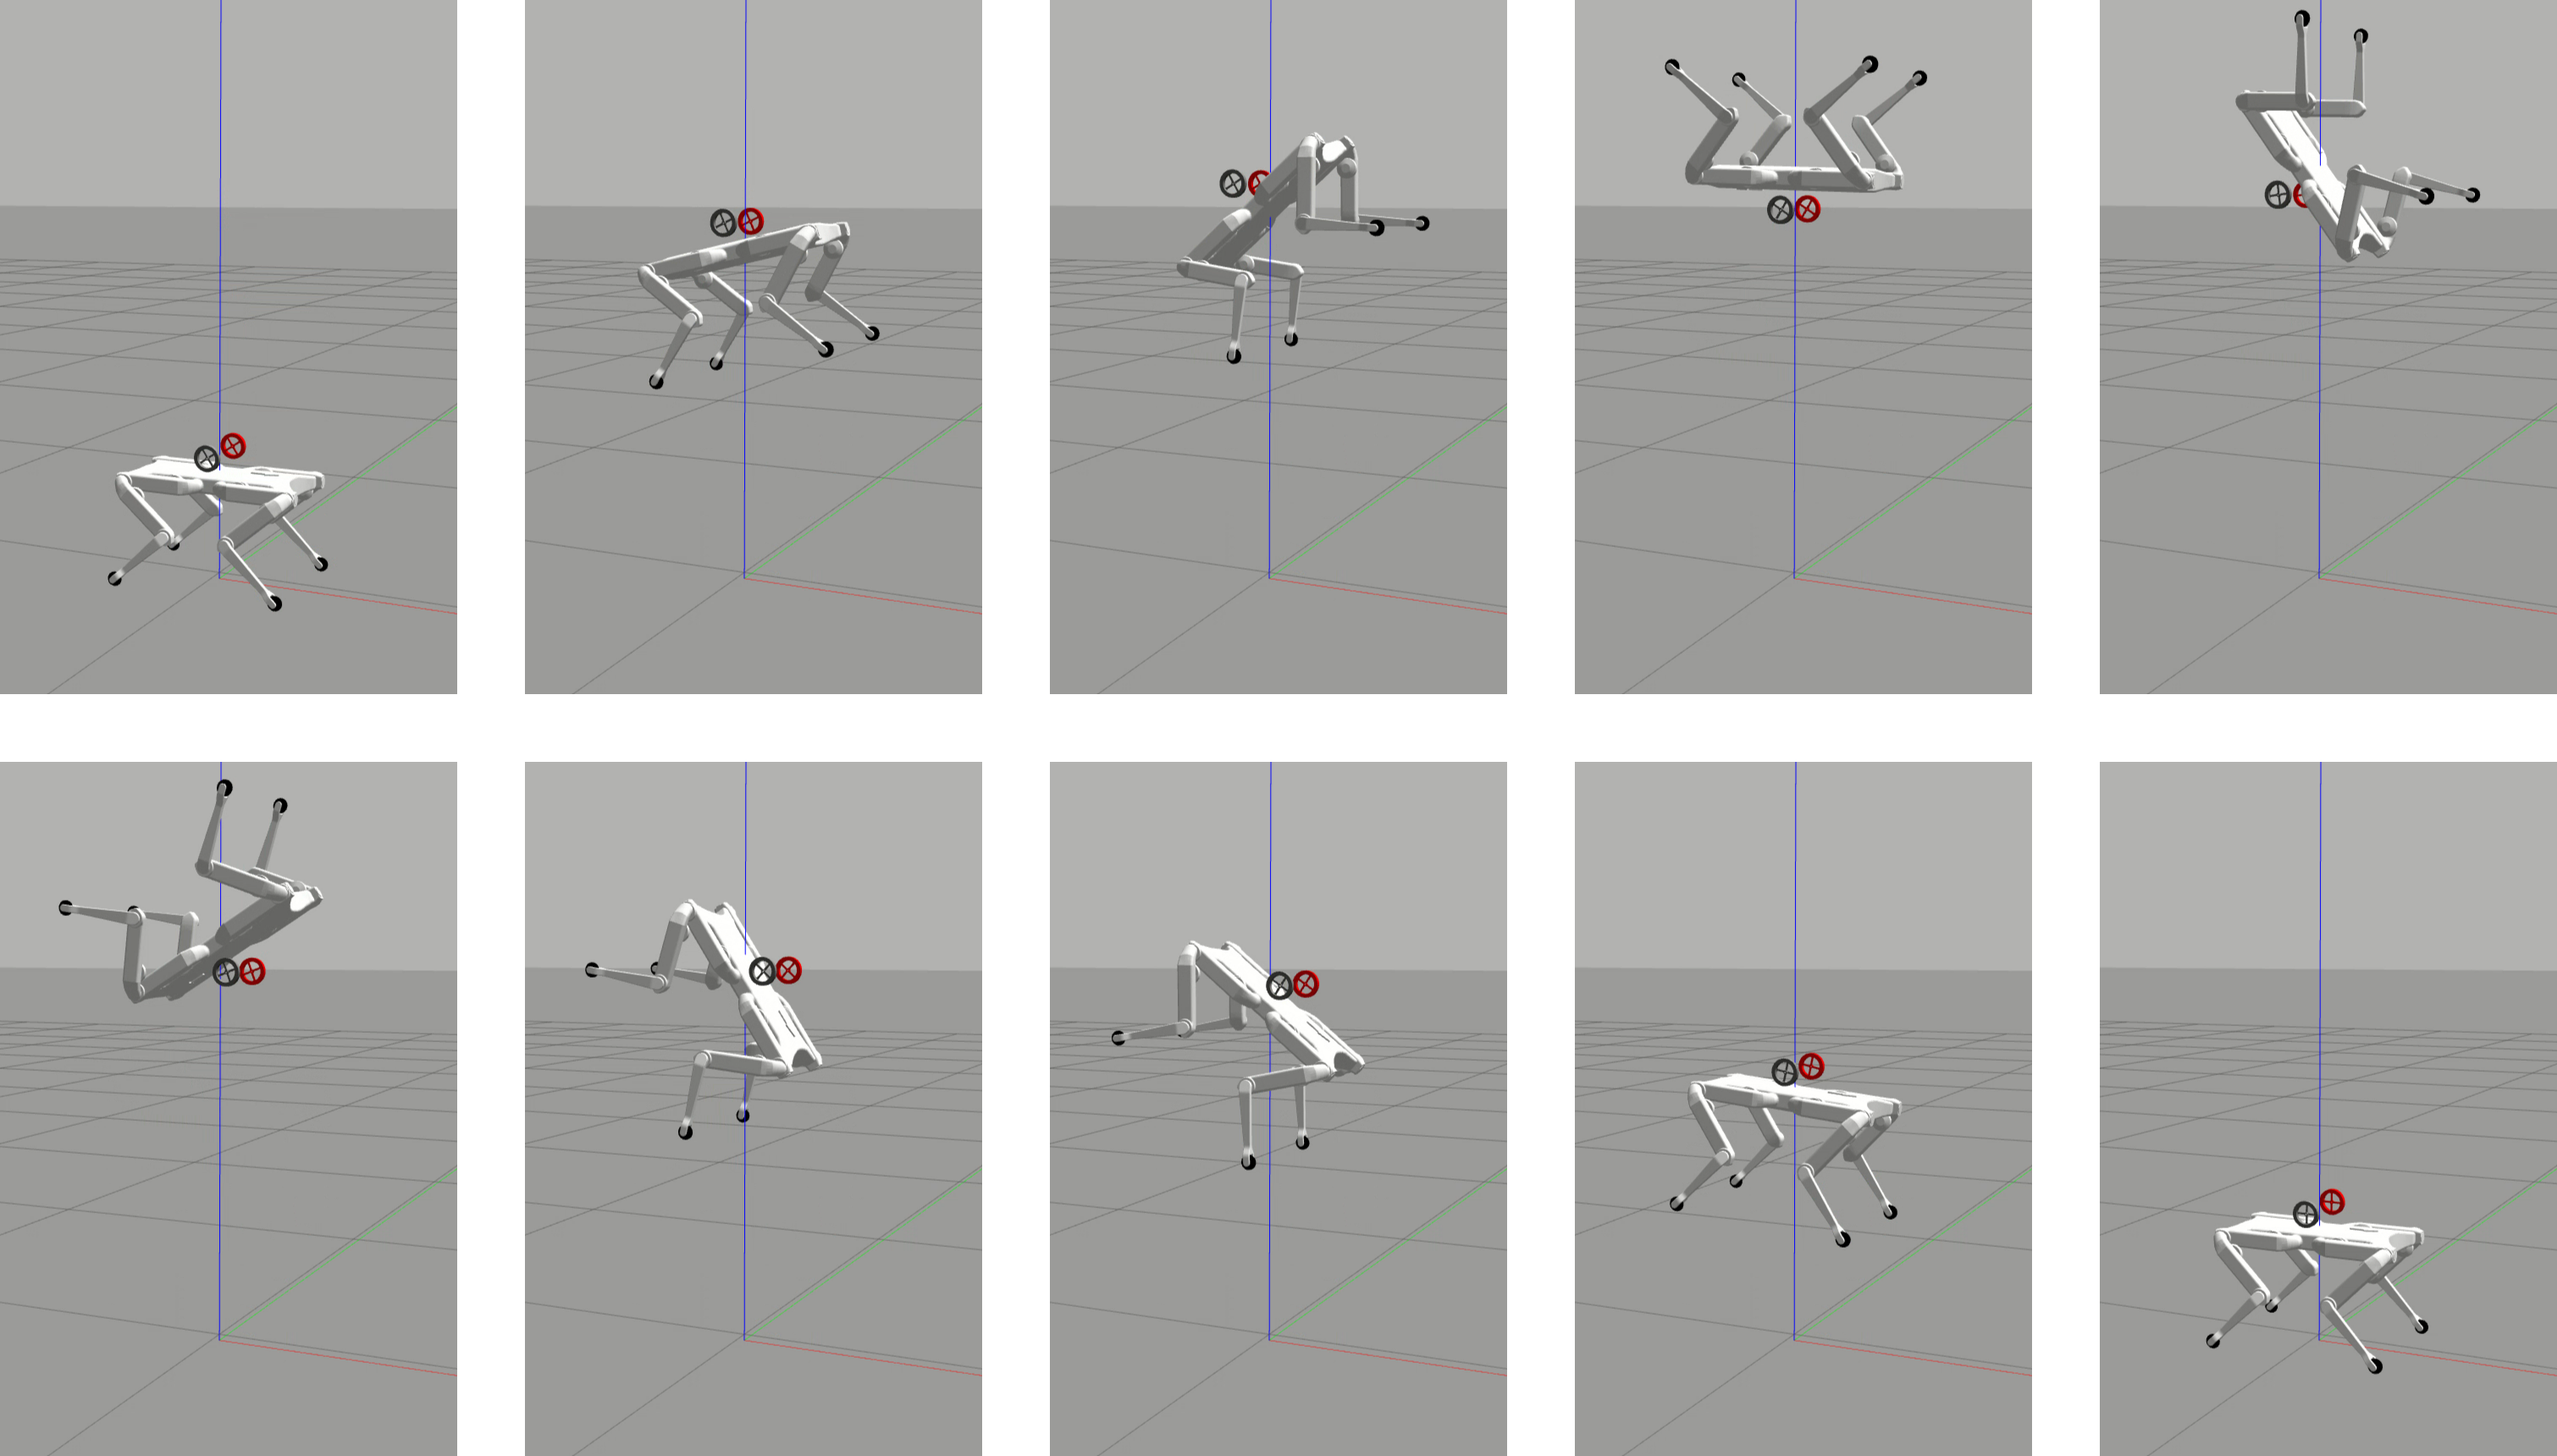
\includegraphics[width=\linewidth]{figures/backflip.png}
		\caption{\small Third Test: sequence of snapshots of Solo12 performing a back-flip in Gazebo environment. The \gls{ocs} alleviates the effort requested to the leg joints, that in this case can be used to accomplish only the vertical motion. The red, green and blue lines represent the axes of the inertial (world) reference frame.}
		\label{fig:backflip}
	\end{figure}
	\begin{table}[H] 
		\caption{Physics related parameters used for simulate the robot dynamics in Gazebo}
		\label{tab:pys_param}
		\newcolumntype{C}{>{\centering\arraybackslash}X}
		\begin{tabularx}{\textwidth}{CC}
			\toprule
			\textbf{Parameter} & \textbf{Value} \\
			\midrule
			Step size & $0.001 \ \mathrm{s}$\\
			Real time update rate & $250$ \\
			Physics engine & Open Dynamics Engine (ODE) \\
			Solver & Quick (Projected Gauss-Seidel method)\\
			Iterations & $50$\\
			Successive Over Relaxation parameter & $1.3$\\
			Rescaling Moment of Inertia  & no \\
			Friction model & Pyramid \\		
			\bottomrule	\end{tabularx}
	\end{table} 
	\item \textbf{Comment 2:} \textit{The authors should give more details regarding the next sentence, being crucial for the paper outputs: "The robot full dynamics is modeled with Pinocchio". Currently Gazebo supports 4 physics engines: ode, bullet, simbody and dart, being the default physics engine ode. Since the simulator models the robot dynamics, why use Pinocchio software?}
	\item[] \textbf{Response:} We acknowledge that we could have made a better explanation here. We rephrased "The robot full dynamics is modeled with Pinocchio. The references for the joints of the legs are computed off-line using Crocoddyl and tracked with a proportional-derivative joint controller." with "References for the joints of the legs are computed off-line using Crocoddyl, an optimal control library for robots based on Differential Dynamic Programming (DDP) algorithms. It uses Pinocchio for fast computation of robots dynamics and their analytical derivatives. References $\bm{q}_{ref}$, $\dot{\bm{q}}_{ref}$ and $\bm{\tau}_{ref}$ for joint positions, velocities and torques are then executed on-line with a proportional-derivative joint controller:
	\begin{equation*}
	\bm{\tau}_j = \bm{K}_{p,\, j} (\bm{q}_{ref} - \bm{q}) + \bm{K}_{d,\, j} (\dot{\bm{q}}_{ref} - \dot{\bm{q}}) + \bm{\tau}_{ref}"
	\end{equation*}
	\item \textbf{Comment 3:} \textit{ Section 2 should be expanded with more citations, an describing more related works.}
	\item[] \textbf{Response:} Thank you for the suggestion. Reviewer 1 pointed out the same advise, then you could refer to the response to Comment 5 of the the previous section. 
	\item \textbf{Comment 4:} \textit{Ide for robot code development}
	\item[] \textbf{Response:} We coded the controller using Python v3.8, with the IDE Pycharm v3.2 (\url{https://www.jetbrains.com/pycharm/}). The manuscript lacks about this information because we believe that, in our work, the use of a specific IDE is not relevant.
\end{itemize}
\vspace{12 pt} 
\noindent In addition to the above observations, all orthographic and grammatical errors mentioned have been corrected.

We look forward to hear regarding our submission and to respond to any further questions and comments.
\vspace{18pt}
\begin{flushright}
	Sincerely,\\
	Michele Focchi, Ph.D.	
\end{flushright}




%%%%%%%%%%%%%%%%%%%%%%%%%%%%%%%%%%%%%%%%%%


%%%%%%%%%%%%%%%%%%%%%%%%%%%%%%%%%%%%%%%%%%
%% optional
%\supplementary{The following supporting information can be downloaded at:  \linksupplementary{s1}, Figure S1: title; Table S1: title; Video S1: title.}

% Only for the journal Methods and Protocols:
% If you wish to submit a video article, please do so with any other supplementary material.
% \supplementary{The following supporting information can be downloaded at: \linksupplementary{s1}, Figure S1: title; Table S1: title; Video S1: title. A supporting video article is available at doi: link.}

%%%%%%%%%%%%%%%%%%%%%%%%%%%%%%%%%%%%%%%%%%
 

%%%%%%%%%%%%%%%%%%%%%%%%%%%%%%%%%%%%%%%%%%
%% Optional
%\appendixtitles{no} % Leave argument "no" if all appendix headings stay EMPTY (then no dot is printed after "Appendix A"). If the appendix sections contain a heading then change the argument to "yes".
%\appendixstart
%\appendix
%\section[\appendixname~\thesection]{}
%\subsection[\appendixname~\thesubsection]{}
%The appendix is an optional section that can contain details and data supplemental to the main text---for example, explanations of experimental details that would disrupt the flow of the main text but nonetheless remain crucial to understanding and reproducing the research shown; figures of replicates for experiments of which representative data are shown in the main text can be added here if brief, or as Supplementary Data. Mathematical proofs of results not central to the paper can be added as an appendix.

%\begin{table}[H] 
%\caption{This is a table caption.\label{tab5}}
%\newcolumntype{C}{>{\centering\arraybackslash}X}
%\begin{tabularx}{\textwidth}{CCC}
%\toprule
%\textbf{Title 1}	& \textbf{Title 2}	& \textbf{Title 3}\\
%\midrule
%Entry 1		& Data			& Data\\
%Entry 2		& Data			& Data\\
%\bottomrule
%\end{tabularx}
%\end{table}

%\section[\appendixname~\thesection]{}
%All appendix sections must be cited in the main text. In the appendices, Figures, Tables, etc. should be labeled, starting with ``A''---e.g., Figure A1, Figure A2, etc.

%%%%%%%%%%%%%%%%%%%%%%%%%%%%%%%%%%%%%%%%%%
%\begin{adjustwidth}{-\extralength}{0cm}
%\printendnotes[custom] % Un-comment to print a list of endnotes

%\reftitle{References}

% Please provide either the correct journal abbreviation (e.g. according to the “List of Title Word Abbreviations” http://www.issn.org/services/online-services/access-to-the-ltwa/) or the full name of the journal.
% Citations and References in Supplementary files are permitted provided that they also appear in the reference list here. 

%=====================================
% References, variant A: external bibliography
%=====================================
%\bibliography{references/bibliography.bib}

%=====================================
% References, variant B: internal bibliography
%=====================================
%\begin{thebibliography}{999}
% Reference 1
%\bibitem[Author1(year)]{ref-journal}
%Author~1, T. The title of the cited article. {\em Journal Abbreviation} {\bf 2008}, {\em 10}, 142--149.
% Reference 2
%\bibitem[Author2(year)]{ref-book1}
%Author~2, L. The title of the cited contribution. In {\em The Book Title}; Editor 1, F., Editor 2, A., Eds.; Publishing House: City, Country, 2007; pp. 32--58.
% Reference 3
%\bibitem[Author3(year)]{ref-book2}
%Author 1, A.; Author 2, B. \textit{Book Title}, 3rd ed.; Publisher: Publisher Location, Country, 2008; pp. 154--196.
% Reference 4
%\bibitem[Author4(year)]{ref-unpublish}
%Author 1, A.B.; Author 2, C. Title of Unpublished Work. \textit{Abbreviated Journal Name} year, \textit{phrase indicating stage of publication (submitted; accepted; in press)}.
% Reference 5
%\bibitem[Author5(year)]{ref-communication}
%Author 1, A.B. (University, City, State, Country); Author 2, C. (Institute, City, State, Country). Personal communication, 2012.
% Reference 6
%\bibitem[Author6(year)]{ref-proceeding}
%Author 1, A.B.; Author 2, C.D.; Author 3, E.F. Title of presentation. In Proceedings of the Name of the Conference, Location of Conference, Country, Date of Conference (Day Month Year); Abstract Number (optional), Pagination (optional).
% Reference 7
%\bibitem[Author7(year)]{ref-thesis}
%Author 1, A.B. Title of Thesis. Level of Thesis, Degree-Granting University, Location of University, Date of Completion.
% Reference 8
%\bibitem[Author8(year)]{ref-url}
%Title of Site. Available online: URL (accessed on Day Month Year).
%\end{thebibliography}

% If authors have biography, please use the format below
%\section*{Short Biography of Authors}
%\bio
%{\raisebox{-0.35cm}{\includegraphics[width=3.5cm,height=5.3cm,clip,keepaspectratio]{Definitions/author1.pdf}}}
%{\textbf{Firstname Lastname} Biography of first author}
%
%\bio
%{\raisebox{-0.35cm}{\includegraphics[width=3.5cm,height=5.3cm,clip,keepaspectratio]{Definitions/author2.jpg}}}
%{\textbf{Firstname Lastname} Biography of second author}

% For the MDPI journals use author-date citation, please follow the formatting guidelines on http://www.mdpi.com/authors/references
% To cite two works by the same author: \citeauthor{ref-journal-1a} (\citeyear{ref-journal-1a}, \citeyear{ref-journal-1b}). This produces: Whittaker (1967, 1975)
% To cite two works by the same author with specific pages: \citeauthor{ref-journal-3a} (\citeyear{ref-journal-3a}, p. 328; \citeyear{ref-journal-3b}, p.475). This produces: Wong (1999, p. 328; 2000, p. 475)

%%%%%%%%%%%%%%%%%%%%%%%%%%%%%%%%%%%%%%%%%%
%% for journal Sci
%\reviewreports{\\
%Reviewer 1 comments and authors’ response\\
%Reviewer 2 comments and authors’ response\\
%Reviewer 3 comments and authors’ response
%}
%%%%%%%%%%%%%%%%%%%%%%%%%%%%%%%%%%%%%%%%%%
%\end{adjustwidth}
\end{document}

